\section{Design}
I dette projekt er der valgt så vidt muligt at designe alle løsninger med diskret elektronik. Derfor er det valgt at forforstærkeren bygges af commonemittertrin med uafkoblet emittermodstand. Et commonemittertrins typiske opbygning er vist på figur \ref{fig:cekobling}.

\begin{figure}[h]
\centering
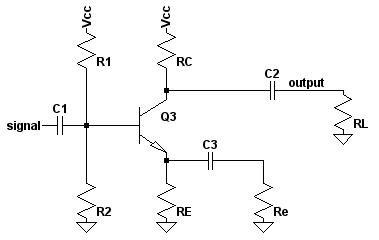
\includegraphics[scale=.6]{teknisk/forforstaerker/ceopkobling.png}
\caption{Generel form på commonemitterkobling med uafkoblet emittermodstand}
\label{fig:cekobling}
\end{figure}


Argumentet for dette valg er at det er det eneste trin, blandt commonemitter, -base og -collector, hvis spændingsforstærkning er betydeligt over én og ikke, under korrekte omstændigheder, afhænger af transistorparametre. Da transistorparametre blandt andet er afhængige af den anvendte transistors temperatur er det en betragtelig styrke ikke at skulle tage højde for dem. Spændingsforstærkningen i commonemittertrinnet er dog kun uafhængig af transistorparametre så længe følgende er gældende: $r_o >>R_C \| R_L$, $gm \cdot R_E||R_e$ og $i_e \approx i_c$.
Dette skyldes at forstærkningen er givet ved ligning (\ref{eq:gmbevis})\fixme{kilde sedra smith eller mm6 AEL}.

\begin{equation}
A_v =  \frac{-gm \cdot R'_L}{1+gm \cdot R'_e} \approx  -\frac{R'_L}{R'_e} \Biggr\vert _{\frac{1}{gm}<<R'_e}
\label{eq:gmbevis}
\end{equation}

Hvor $R'_e = R_e || R_E$ og $R'_L = R_L||R_C$. Det vil sige at jo tættere $R_e$ kommer på $\frac{1}{gm}$ jo mere indflydelse vil denne have på forstærkningen. Disse antagelser vil derfor være gældende gennem hele designet af forforstærkeren. 

Det første trin skal have en forstærkning på 10 gange og det andet på 6,97 for at opnå den ønskede forstærkning, som vist på figur \ref{blok_forforstaerker}. Grunden til rækkefølgen af trinnene er for ikke at have størst signaludsving og den største forstærkning i samme trin. Dette skyldes at der i en forstærker altid vil være forvrængning og støj. Hvis den største forstærkning kommer sidst, vil denne forvrængning blive forstærket yderligere, hvilket ikke er ønskværdigt. Hvis den største forstærkning derimod kommer først, vil der blive mindst muligt forvrængning med i det endelige signal.\fixme{Hvordan viser vi at det er smart? Frederik: Er det godt nok? Skal der skrives mere? Skal der beregninger med, der beviser det? (synes jeg ikke)}

\begin{figure}[h]
\centering
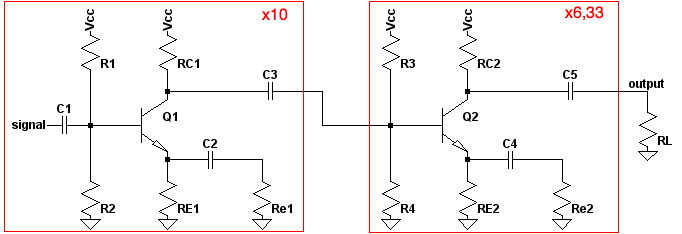
\includegraphics[scale=.6]{teknisk/forforstaerker/blok_forforstaerker.png}
\caption{Blokdiagram over forforstærkerens byggeblokke samt lydsignalets vej}
\label{blok_forforstaerker}
\end{figure}

For at opnå så lav forvrængning som muligt designes hvert trin således at forstærkningen, uden den AC-koblede emittermodstand $R_e$, er så stor som muligt for at gøre tilbagekobling muligt. For derefter at få den ønskede forstærkning tilføjes tilbagekoblingsmodstanden $R_e$.

\subsection*{Design af første trin}
Begge trin designes efter maksimal forstærkning uden $R_e$. Denne forstærkning er givet ved ligning (\ref{eq:dcgain}).

\begin{equation}
|A_{vs}|=\frac{1}{\left(\frac{V_T \cdot R_C}{V_{R_C}}+\frac{R'_S}{\beta}\right) \left(\frac{1}{R_C}+\frac{1}{R_L}\right)}
\label{eq:dcgain}
\end{equation}
Hvor $R'_S = R_S||R_1||R_2$ og $V_T = 26 \cdot 10^{-3}$.

For at designe et kredsløb med maksimal forstærkning justeres størrelsen af $R_C$ uden at variere spændingen over den, $V_{R_C}$. Den maksimale $R_C$ findes ved ligning (\ref{eq:rcmaks}).

\begin{equation}
R_{\mathrm{C,maks}} = \sqrt{\frac{R'_S \cdot R_L \cdot V_{R_C}}{\beta \cdot V_T}}
\label{eq:rcmaks}
\end{equation}

I ligning (\ref{eq:rcmaks}) er $R'_S$ defineret som $R_1||R_2||R_S$. $R_S$ er fastlagt til 2,2 k\ohm, hvilket er mikrofonens udgangsimpedans\fixme{kilde til MCE4000}. Parallelforbindelsen mellem $R_1$ og $R_2$ kan ikke beregnes men skal vælges. Indgangsimpedansen i kredsløbet, som netop er $R_1||R_2$, skal som hovedregel være meget større end udgangsimpedansen i den kreds den belaster. En tommelfingerregel siger at 10 gange større er tilstrækkeligt til at være $"$meget større$"$ hvormed parallelkoblingen skal være over eller lig med 22 k\ohm. 
Belastningen, $R_L$, for det første trin bliver indgangsimpedansen i det andet. Indgangsimpedansen i det andet trin bliver $R_3||R_4$ og kan heller ikke beregnes. Da $R_C$ i det første trin ikke kendes endnu vælges indgangsimpedansen i det andet til at være den samme som i det første, altså 22 k\ohm. 
$V_{R_C}$ er defineret som værende $V_{CC} - V_{\mathrm{CE,sat}} - V_{R_E} - V_{\mathrm{o,peak}}$, hvor $V_{CC}$ vælges til 15 V så der sikres at der er plads til det ønskede spændingsudsving, $V_{R_E}$ vælges til 3 V og $V_{\mathrm{CE,sat}}$ aflæses i databladet for BC547b til 0,2 V ved en collectorstrøm på 1 mA. Der antages at collectorstrømmen cirka bliver 1 mA. Ligeledes aflæses $\beta$ til 250 ved 1 mA i databladet. $V_{\mathrm{o,peak}}$ er peakspændingen på udgangen. Dermed bliver peakspændingen en faktor 10 højere end mikrofonens output peakspænding. $V_{\mathrm{o,peak}}$ bliver derfor 316 mV. $R_{C1}$ beregnes hermed i ligning (\ref{eq:rcforsteberegning}).

\begin{equation}
R_{\mathrm{C1}} = \sqrt{\frac{22~k\ohm || 2,2~k\ohm \cdot (15~V - 0,2~V - 3~V - 0,287~V)}{250 \cdot 26 \cdot 10^{-3}}}=8,83~k\ohm
\label{eq:rcforsteberegning}
\end{equation}

$R_{E1}$ bestemmes i ligning (\ref{eq:beregningre1}) under antagelse at $i_e = i_c$.  $i_c$ beregnes i ligning(\ref{eq:ff:ic}).

\begin{equation}
\label{eq:ff:ic}
i_C=\frac{V_{R_C}}{R_C}=\frac{11,5~V}{9,25~k\ohm}=106,4~mA
\end{equation}
\begin{equation}
R_{E1}=\frac{V_{R_{E1}}}{\frac{V_{R_{C1}}}{R_{C1}}}  \Rightarrow R_{E1}=\frac{3~V}{106,4~mA}=2,30~k\ohm
\label{eq:beregningre1}
\end{equation}


Dernæst beregnes $R_{e1}$ ud fra hvad den ønskede forstærkning skal være. Ligning (\ref{eq:gmbevis}) benyttes til at beregne $R_{e1}$ i ligning (\ref{eq:rlilleeberegning}).

\begin{equation}
\label{eq:rlilleeberegning}
A_v = -\frac{R'_L}{R'_e} \Rightarrow  R_{e1} =-\frac{R_L \cdot R_{C1} \cdot R_{E1}}{A_v \cdot R_{E1} \cdot R_{C1} + A_v \cdot R_{E1} \cdot R_L + R_{C1} \cdot R_L} \Rightarrow R_{e1} = 867,6~\ohm
\end{equation}

Biasnetværket, bestående af $R_1$ og $R_2$ beregnes ud fra den spænding, som er påkrævet på basen for at transistoren fungerer som ønsket. Spændingen over base-emitter, $V_{\mathrm{BE}}$ er i databladet aflæst til 0,6 V. Da potentialet på emitteren er 3 V skal potentialet på basen være 3,6 V. $R_1$ og $R_2$ kan beregnes ud fra at $V_{R_2}$ skal være 3,6 V og parallelkoblingen $R_1||R_2$. Beregningen udføres i ligning (\ref{eq:r1r21}) og (\ref{eq:r1r22}).

\begin{equation}
V_{R_2} = V_{CC} \cdot \frac{R_2}{R_1+R_2} 
\label{eq:r1r21}
\end{equation}
\begin{equation}
R_1||R_2 = \frac{R_1 \cdot R_2}{R_1 + R_2}
\label{eq:r1r22}
\end{equation}
De kendte værdier indsættes og de to ligninger med to ubekendte løses. Resultatet er vist i ligning (\ref{eq:r1r2result}).
\begin{equation}
R_1 = 91,7~k\ohm ~ \wedge ~ R_2=28,9~k\ohm
\label{eq:r1r2result}
\end{equation}

For at opnå den ønskede frekvensgang skal $C1$, $C2$ og $C3$ dimensioneres således at den knækfrekvens de hver især frembringer. Da knækfrekvensen er det punkt hvor kurven er faldet 3 dB og frekvensgangen skal, jævnfør kravspecifikationen, være 20 Hz til 20 kHz, er det nødvendigt at knækfrekvens  ligger før 20 Hz. Det vurderes at knækfrekvensen beregnes til at ligge i 2 Hz for at knækfrekvensen ikke giver anledning til en dæmpning af signalet på mere end de tilladte 3 dB.

Kondensatorerne beregnes med formel (\ref{eq:kondensatorknaek}).

\begin{equation}
C=\frac{1}{\omega \cdot R}=\frac{1}{2\cdot \pi \cdot f \cdot R}
\label{eq:kondensatorknaek}
\end{equation}

I ligning \ref{eq:kondensatorknaek} er $C$ kondensatorens capacitet og $R$ er den impedans kondensatoren ser ind i. 
$C1$ ser ind i forspændingskoblingen i det første forstærkertrin, altså 22 k\Ohm. $C2$ ser ind i den AC-koblede emittermodstand, $Re1$. $C3$ ser ind i forspændingsnetværket i det andet forstærkertrin, altså 22 k\Ohm. Dermed bliver kondensatorernes værdier som følger.

\begin{equation}
C1=3,58~\my F~\wedge ~C2=91,9~\my F~\wedge ~C3=3,58~\my F
\end{equation}



\subsection*{Design af andet trin}
Beregning af andet trin følger samme designprocedure som første trin. Kredsløbet til andet trin er vist på figur \ref{fig:andettrinkreds}.

\begin{figure}[h]
\centering
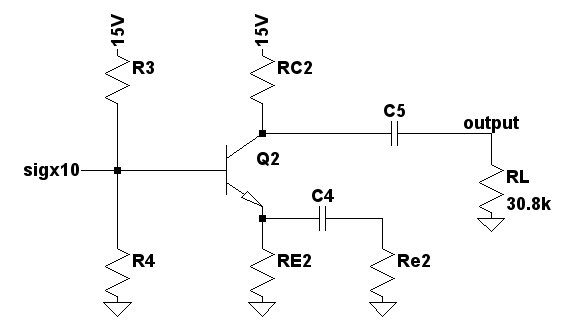
\includegraphics[scale=.6]{teknisk/forforstaerker/andettrinkreds.png}
\caption{Det andet trins kredsløb}
\label{fig:andettrinkreds}
\end{figure}

Det andet trin skal forstærke et signal med en maksimal peakspænding på 287 mV op til 2 V, altså 6,97 gange. Belastningsmodstanden for dette forstærkertrin er bestemt af indgangsvælgeren, som er det næste trin efter forforstærkeren. Indgangsvælgerens indgangsimpedans er 30,8 k\ohm \fixme{reference til indgangsvælgeren hvor det står}. $R_S$ er i dette trin givet ved udgangsmodstanden for det første forstærkertrin, som er lig med $R_{C1}$ hvilket gør at $R'_S = R_{C1} || R_3 || R_4$. Den maksimale $R_{C2}$ beregnes i ligning \ref{eq:rc2maks}.

\begin{equation}
R_{\mathrm{C2}} = \sqrt{\frac{R'_S \cdot R_L \cdot V_{R_C2}}{\beta \cdot V_T}} = 17,1~k\ohm
\label{eq:rc2maks}
\end{equation}

Beregningerne af $R_{E2}$ og $R_{e2}$ samt kondensatorerne er meget ens med dem for det første forstærkertrin. Derfor er det valgt ikke at vise beregningerne i rapporten. $R_3$ og $R_2$ antager samme værdier som henholdsvis $R_1$ og $R_2$, da begge trin skal have samme indgangsimpedans. De beregnede værdier er vist i ligning (\ref{eq:valuestrin2}).

\begin{equation}
R_{E2}=5233,7~\ohm ~ \wedge ~R_{e2}=2599,4~\ohm ~ \wedge ~ C4=30,6~\my F ~ \wedge ~ C5=2,6~\my F
\label{eq:valuestrin2}
\end{equation}

Det endelige kredsløb er vist på figur \ref{fig:forforstaerkersimuleringkredslob} i simuleringsafsnittet.

\subsection*{Simulering}

For at verificere at kredsløbet fungerer som ønsket simuleres det i LTspice. De karakteristika som skal verificeres er spændingsforstærkningen, amplitudekarakteristikken samt harmonisk forvrængning. Kredsløbet der simuleres er vist på figur \ref{fig:forforstaerkersimuleringkredslob}. På figuren er der til alle komponenter angivet en beregnet værdi, som den øverste, og en tilsvarende værdi i modstandsrækken E96. 

\begin{figure}[h]
\centering
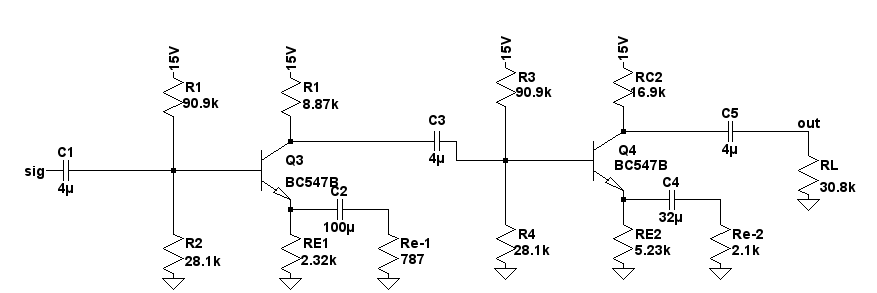
\includegraphics[scale=.6]{teknisk/forforstaerker/forforstaerkerendeligkreds.png}
\caption{}
\label{}
\end{figure}

Kredsløbet simuleres med modstandsværdierne hørende til E96 rækken fordi det er de værdier der i praksis skal bruges til at bygge den endelige forforstærker. 
Spændingsforstærkningen af hele trinnet skal være 69,7 gange svarende til 36,9 dB. Forstærkningen vises på figur \ref{fig:amplitude-forforstaerker} ved hjælp af en amplitudekarakteristik, således at spændet fra 20 Hz til 20 kHz tydeligt kan ses. 


\begin{figure}[h]
\centering
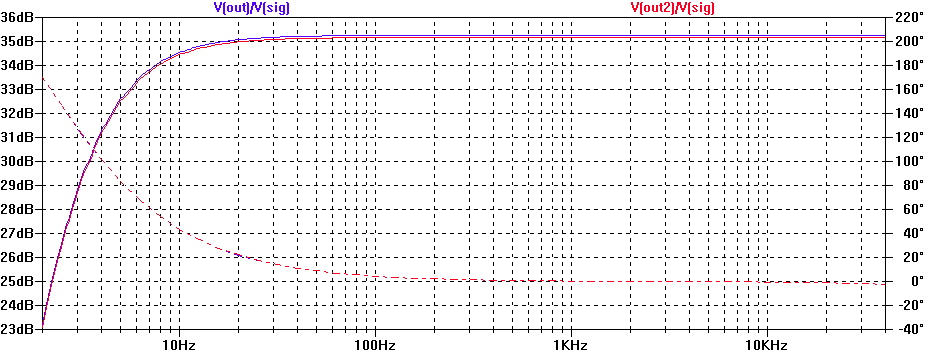
\includegraphics[scale=.6]{teknisk/forforstaerker/amplitudeforforstaerker.png}
\caption{Forforstærkerens amplitude karakteristik}
\label{fig:amplitude-forforstaerker}
\end{figure}

Simuleringen viser at forstærkningen ved 1 kHz, som er referencen jævnfør kravspecifikationen, er 36 dB hvor den skulle have være 36,9 dB. Dermed må der konkluderes at beregningen af forforstærkertrinnene indeholder usikkerheder. Usikkerhederne vurderes til at bestå i de antagelser som defineres før beregningerne: $r_o >>R_C \| R_L$, $gm \cdot R_E||R_e$ og $i_e \approx i_c$. For at korrigere forstærkningen i trinnene kan der, ifølge ligning \ref{eq:gmbevis}, justeres på den AC-koblede emittermodstand, $R_{e1}$ og $R_{e2}$. I ligning \ref{eq:nyerevalues} er de nye værdier for disse modstanden anvist. Disse modstanden er fundet ved først at justere $R_{e1}$ til det første trin giver den korrekte forstærkning for derefter at gøre det samme med det andet trin.

\begin{equation}
R_{e1}=790~\ohm~\wedge ~R_{e2}=2,1~k\ohm
\label{eq:nyerevalues}
\end{equation}

Med de nye modstandsværdier bliver amplituden som vist på figur \ref{fig:rigtigamplitudeforforstaerker}.

\begin{figure}[h]
\centering
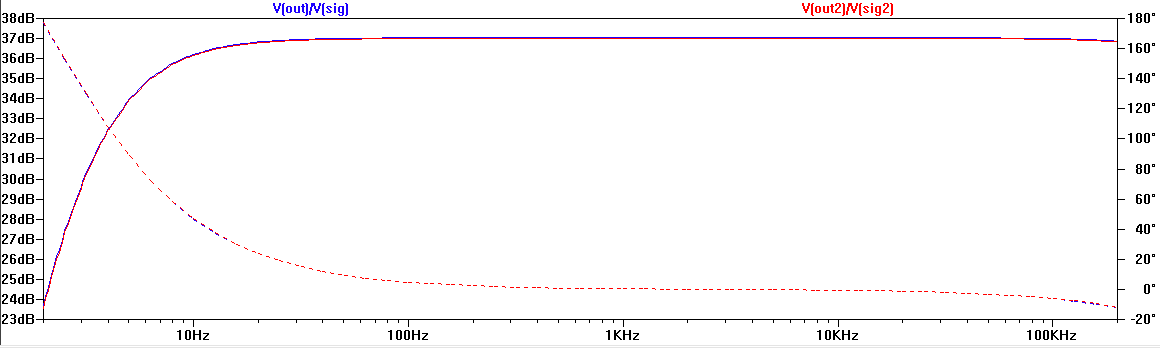
\includegraphics[scale=.6]{teknisk/forforstaerker/rigtigamplitude.png}
\caption{Forforstærkerens amplitudekarakteristik efter korrektion af forstærkning}
\label{fig:rigtigamplitudeforforstaerker}
\end{figure}

På figur \ref{fig:rigtigamplitudeforforstaerker} ses det at forstærkningen nu er korrigeret. Derudover fremgår det at dæmpningen fra 20 kHz til 20 Hz er 0,2 dB. Dermed overholdes kravet om at dæmpningen i dette område, som skal være under 0,375 dB. 

Den harmoniske forvrængning skal ifølge kravspecifikationen være under 0,5 \%. Ifølge LTspice er den harmoniske forvrængning ved 1 kHz og maksimal peakspænding på indgangen 0,18 \%. Forvrængningsmålingen er udført ved maksimal peakspænding da forvrængningen i trinnet vil være mest kritisk i den situation. 






